\begin{pastexam}[label={px:ncku-114-isec-ds-08}]{成大智慧資安學程 114 學年度 單選題第 8 題}
（單選；每題 5 分，答錯倒扣 2 分）

Prim algorithm is used to construct a minimum spanning tree $T$ by using the data structure ``set''.
They form a set for all nodes in the beginning and gradually merge two nodes until $T$ is found. Please
identify the first edge which form a cycle in $T$ during the procedure and the number of sets formed at
that moment.

\begin{center}
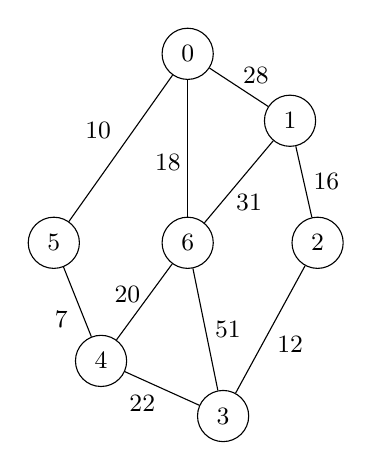
\begin{tikzpicture}[v/.style={draw,circle,minimum size=6.5mm,inner sep=0pt},font=\small]
  \node[v] (0) at (0,0) {0};
  \node[v] (1) at (1.3,-0.85) {1};
  \node[v] (5) at (-1.7,-2.4) {5};
  \node[v] (6) at (0,-2.4) {6};
  \node[v] (2) at (1.65,-2.4) {2};
  \node[v] (4) at (-1.1,-3.9) {4};
  \node[v] (3) at (0.45,-4.6) {3};
  \draw (0) -- node[above right=-2pt] {28} (1);
  \draw (0) -- node[above left] {10} (5);
  \draw (0) -- node[left=-1pt,pos=0.6] {18} (6);
  \draw (1) -- node[below right=-2pt,pos=0.6] {31} (6);
  \draw (1) -- node[right] {16} (2);
  \draw (5) -- node[below left] {7} (4);
  \draw (6) -- node[left,pos=0.4] {20} (4);
  \draw (6) -- node[right] {51} (3);
  \draw (2) -- node[below right=-1pt] {12} (3);
  \draw (4) -- node[below left=-1pt] {22} (3);
\end{tikzpicture}
\end{center}

a)~edge (3, 6) and 2 set \qquad b)~edge (4, 6) and 4 set

c)~edge (0, 1) and 3 set \qquad d)~edge (4, 6) and 3 set

e)~None of the above
\end{pastexam}

\begin{pastsoln}
答案是 b) edge (4, 6) and 4 set（照題目說的 Prim 演算法、從頂點 0 開始）。

\textbf{題目的歧義。} 題目寫 Prim，但「一開始每個點自成一個集合、逐步合併」是 Kruskal 的描述（資結書
第~24.2~節），兩種讀法答案不同，下面兩種都算。 Prim 沒有指定起點，取編號最小的 $0$。 把 Prim 也用
「集合」來看：長出來的樹是一個集合，還沒加進來的頂點各自一個集合。

\textbf{照 Prim，從 0 開始}（資結書第~24.3~節）。 每一步從「一端在樹裡、一端在樹外」的邊中挑最輕的；
用候選邊的優先佇列實作時，佇列裡的邊可能兩端後來都進了樹，取出時就會形成迴圈，要丟掉
（資結書虛擬碼~24.4 的作法）。
\begin{center}
\small
\begin{tabular}{llll}
\toprule
步 & 取出的最輕候選邊 & 結果 & 樹 \\
\midrule
1 & $(0, 5)$ 10 & 加入 & $\{0, 5\}$ \\
2 & $(5, 4)$ 7 & 加入 & $\{0, 4, 5\}$ \\
3 & $(0, 6)$ 18 & 加入 & $\{0, 4, 5, 6\}$ \\
4 & $(4, 6)$ 20 & 兩端都在樹裡，形成迴圈 & \\
\bottomrule
\end{tabular}
\end{center}
第 2 步時候選邊是 $(0, 1)$ 28、$(0, 6)$ 18、$(5, 4)$ 7、取最輕的 $7$；第 3 步候選邊加上 $(4, 6)$ 20、
$(4, 3)$ 22，最輕的是 $(0, 6)$ 18。 加入 $6$ 之後，最輕的候選邊是 $(4, 6)$ 20，但 $4$、$6$ 都已經在樹裡，
這是第一條形成迴圈的邊。 這時的集合：樹 $\{0, 4, 5, 6\}$ 一個，$\{1\}$、$\{2\}$、$\{3\}$ 各一個，共
$4$ 個。 對應 b)。 （起點取 $4$、$5$、$6$ 也得到同樣的結果；起點取 $1$、$2$、$3$ 時，到 $(4, 6)$ 形成迴圈
時所有頂點都已經進樹，只剩 $1$ 個集合。）

\textbf{若照 Kruskal 的讀法}（邊由輕到重：$7, 10, 12, 16, 18, 20, \dots$）：
\begin{center}
\small
\begin{tabular}{lll}
\toprule
邊 & 結果 & 集合 \\
\midrule
$(4, 5)$ 7 & 加入 & $\{4, 5\}$、其餘各自一個，共 6 個 \\
$(0, 5)$ 10 & 加入 & $\{0, 4, 5\}$，共 5 個 \\
$(2, 3)$ 12 & 加入 & $\{2, 3\}$，共 4 個 \\
$(1, 2)$ 16 & 加入 & $\{1, 2, 3\}$，共 3 個 \\
$(0, 6)$ 18 & 加入 & $\{0, 4, 5, 6\}$、$\{1, 2, 3\}$，共 2 個 \\
$(4, 6)$ 20 & $4$、$6$ 同一個集合，形成迴圈 & 2 個 \\
\bottomrule
\end{tabular}
\end{center}
第一條形成迴圈的邊一樣是 $(4, 6)$，但這時只剩 $2$ 個集合，選項裡沒有「$(4, 6)$ and 2 set」，要選 e)。

兩種讀法第一條成環的邊都是 $(4, 6)$，差別在集合數。 題目明寫 Prim，選項 b) 也恰好是 Prim 從 $0$
開始的結果，所以本書取 b)。 作答時最好註明採用哪種讀法。
\end{pastsoln}
